% !TeX root = ../summary-syssec.tex

\section{Security on Commodity Systems}
\subsection{Application Security}
\subsubsection{Properties}
\begin{description}
  \item[Launch-time integrity:] \textit{correct} application was started
  \item[Run-time isolation:] no interference from malicious software or
    peripherals
  \item[Secure persistent storage] Confidentiality, integrity protection of
    data
\end{description}


\subsection{OS-based Security}
\subsubsection{Privilege Rings}
\begin{center}
  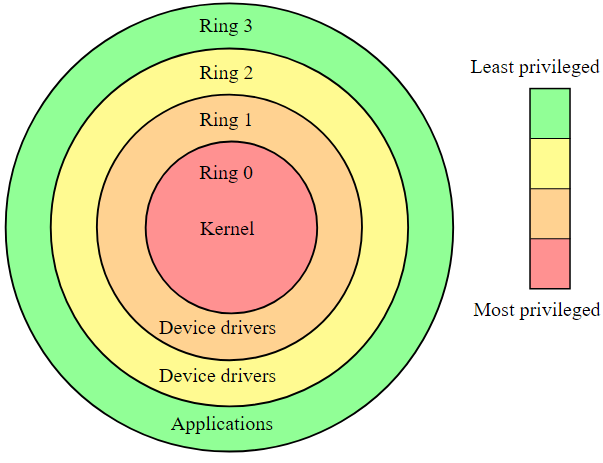
\includegraphics[width = 0.6\columnwidth]{commodity_systems_privilege-rings.png}
\end{center}
\begin{itemize}
  \item Today, only rings 0 and 3 are used; 1 - 2 part of kernel
  \item Main use: limiting access to privileged instructions, I/O-ports
\end{itemize}


\subsubsection{Paging-based Security}
Security-relevant data in page table entries:
\begin{description}
  \item[Supervisor bit:] if set, this page is accessible only in ring 0
    (isolates OS from applications)
  \item[RW bits:] to distinguish between read-only and writeable pages
  \item[Execution disable (ED) bit:] if set, the page is not executable
    (prevents run-time code injection)
\end{description}


\subsubsection{Firewire (DMA) Attack}
\begin{description}
  \item[Background:] Firewire  allows for fast communication speeds
    between devices, uses DMA (Direct Memory Access)
  \item[Idea:] Access to RAM is controlled by CPU. This can be circumvented by
    DMA.
  \item[Attack:]\hfill
    \begin{itemize}
      \item The attacker uses a Firewire cable to connect to a (locked) PC
	and issue a DMA request to fetch the contents of RAM
      \item Later on it can look in the collected data and find out keys and
	other passwords
    \end{itemize}
  \item[Protection:] \hfill
    \begin{itemize}
      \item Have no Firewire ports, but there are other ports for
	similar attacks.
      \item OS sets up a IOMMU (Input–output memory management unit) to control
	DMA access to physical memory.
    \end{itemize}
\end{description}


\subsubsection{Disk Encryption}
\begin{description}
  \item[Idea:] Disk is encrypted and unlocked by a secret key.
    \begin{itemize}
      \item Data on disk is allways encrypted.
      \item File system is completely unaware:
	\begin{center}
	  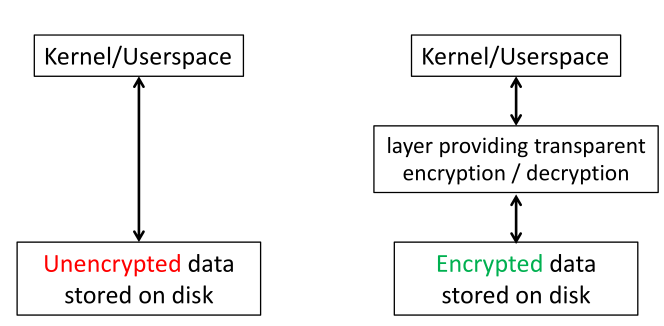
\includegraphics[width=0.6\columnwidth]{commodity_systems_disk-encryption.png}
	\end{center}
    \end{itemize}

  \item[Simple Approach:] Use password only $\Rightarrow$ can be
    bruteforced
  \item[Better Approach:] Store disk encryption key in a secure element
    (TPM) $\Rightarrow$ requires more hardware support.
\end{description}


\subsubsection{Cold Boot Attack on Disk Encryption}
\begin{description}
  \item[Idea:] \hfill
    \begin{itemize}
      \item encryption key is kept in memory
      \item DRAM keeps it's state for a while without refresh, and
	longer if it is cold.
    \end{itemize}
  \item[Attack:] \hfill
    \begin{itemize}
      \item Remove power
      \item Cool down RAM
      \item Plug RAM to another platform / Boot with a USB and attack
	tools to copy memory content
      \item Recover key (part in memory with high entropy)
    \end{itemize}
  \item[Protection:] \hfill
    \begin{itemize}
      \item Erase key from memory on every suspend
	\begin{itemize}
	  \item does not help sudden power loss
	\end{itemize}
      \item Physical protection
      \item Avoid to have key in memory
    \end{itemize}
\end{description}


\subsubsection{Chain of Trust}
\begin{center}
  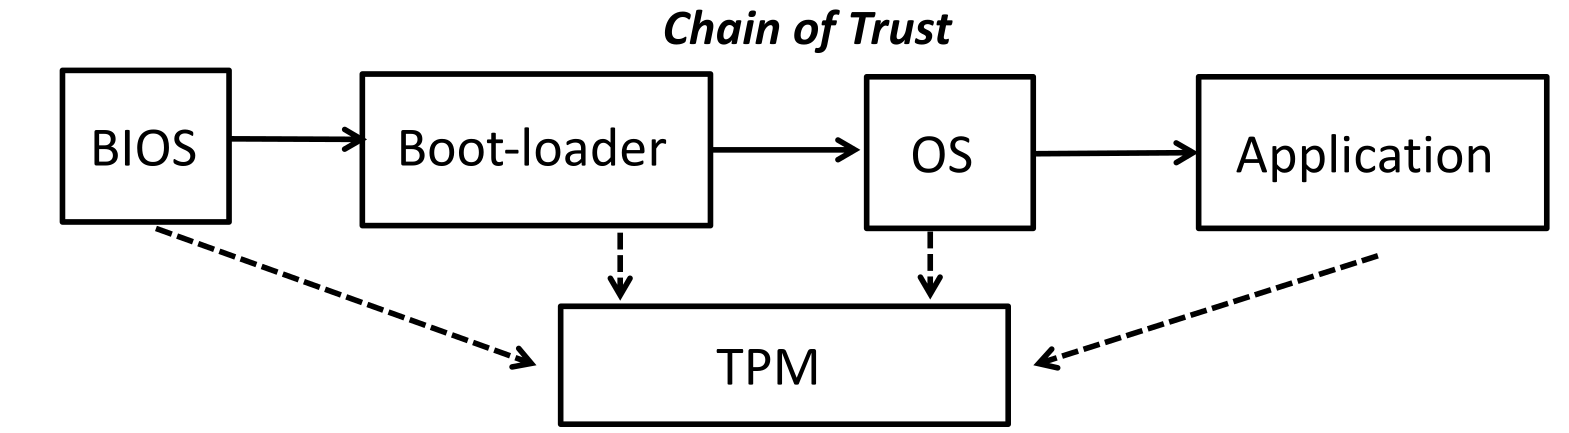
\includegraphics[width=0.7\columnwidth]{commodity_systems_chain-of-trust.png}
\end{center}
\begin{description}
  \item[Secure Boot:] OS boots only if the chain of trust is valid
  \item[Authenticated boot:] System records chain of trust but OS boots
    even if the chain is invalid
\end{description}


\subsection{Storage protection on smartphones}
\subsubsection{Background}
\begin{itemize}
  \item Encrypt with user-provided PIN
  \item no TPM available
  \item Approach:
    \begin{enumerate}
      \item At boot the OS asks PIN code from user
      \item PIN is given to the CPU
      \item CPU derives storage encryption key from PIN and processor key
    \end{enumerate}
    $\Rightarrow$ Prevents brute-forcing of extracted storage
  \item storage must be decrypted on the same device where the CPU is
  \item A counter indicates how many attempts are left.
\end{itemize}

\subsubsection{NAND Mirroring Attack}
\begin{enumerate}
  \item  Eavesdropping:\\
    Find the communication protocols and the communication speeds
  \item Backing Up:\\
    Create a copy of the NAND chip
  \item Restoring:
    \begin{itemize}
      \item Power on phone
      \item Enter 6 PINs
      \item Power down
      \item Take out NAND and restore modified parts from backup
      \item Put NAND back into phone
      \item Repeat
    \end{itemize}
  \item OR Cloning:
    \begin{itemize}
      \item Arbitrarily many clones can be created
      \item Always plug in a new cloned chip
    \end{itemize}
\end{enumerate}
Allows brute-forcing of a 4-digit PIN in less than a day.
